\subsubsection{Ladning}
\paragraph{Atomet} \mbox{} \\
Vi vet fra ungdomsskolen at atomer består av protoner, nøytroner og elektroner.
Elektronene $e^-$ er negativt ladet og protonene $p^+$ positivt.
Protoner og nøytroner er i atomets kjerne, mens elektronene ligger i
"yttre skall".
\\
Et ion er et atom med enten flere elektroner enn protoner, eller motsatt.
Hvis det er flertall av elektroner kalles ionet negativt ladet.
\\
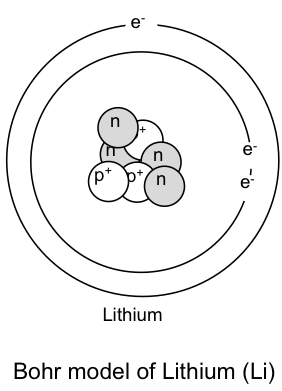
\includegraphics{./img/Li}

\paragraph{Enhet} \mbox{} \\
SI enheten for ladning er Coulomb (C). \hfill $\SI{1}{\coulomb} = 6.24 \times 10^{18}$e\\
Hvor e står for elementærladning, den elektriske ladningen til et proton.
